\chapter{Introducción}
\label{chapter:introduccion}


%%% SECTION
\section{Contexto y justificación del Trabajo}
Cada vez se encuentran más dispositivos conectados entre sí, no solo en la industria, sino también en los hogares, esta conexión entre dispositivos los hace vulnerables a ataques informáticos que pueden afectar en gran medida a los usuarios, no solo pueden provocar un mal funcionamiento de los mismos, sino que también puede provocar la fuga de datos de distinta sensibilidad. La previsión en los futuros años es estar cada vez más conectados y una pronta detección de los ataques puede ayudar a evitar los problemas derivados de los mismos, mediante una pronta reacción o haciendo frente a la previsión de un ataque.



Actualmente se utilizan distintas medidas de seguridad como control de acceso físico al dispositivo, encriptación de datos, firewalls, securización de red, etc... Sin embargo, en muchos casos la detección de anomalías aplica un umbral estacionario, provocando que en el caso de un ataque ya sea demasiado tarde para reaccionar o no se sea capaz de identificar patrones extraños previos al ataque. Con la aplicación de nuevas técnicas se pretende mejorar los tiempos de reacción e incluso predecir cuándo puede suceder un ataque.

\section{Explicación de la motivación personal}
La razón principal de la elección del proyecto es la posibilidad de aprender y utilizar técnicas de Machine Learning en un sector desconocido que permita diversificar conocimientos. Todo se encuentra cada vez más conectado e investigar cómo clasificar cuando se está produciendo un ataque permite profundizar en conocimientos de seguridad y aplicarlos en un problema real.



La aplicación de técnicas en un problema real ayuda a comprender mejor el uso de las herramientas y el porqué y cuándo se deben de utilizar. De este modo, se añade un nuevo conocimiento que aportar al ámbito profesional y puede utilizarse también en un entorno privado.


\section{Objetivos del Trabajo}
Los objetivos del trabajo son los siguientes:

\begin{itemize}
  \item Adquisición de conocimiento del sector y de los dispositivos IOT.
  \item Lectura y comprensión de las técnicas del estado del arte en detección de anomalías en dispositivos conectados.
  \item Obtención de datos reales de conexiones a dispositivos IOT, en caso de no ser posible, generación de datos sintéticos.
  \item Prueba de las técnicas encontradas y evaluación en el problema actual.
  \item Investigación de algoritmos tradicionales de Machine Learning y su utilidad.
  \item Desarrollo de la solución utilizando los algoritmos más aptos.
  \item Evaluación de la detección de patrones y ataques de las técnicas utilizadas.
  \item Comparación de los resultados obtenidos con el estado del arte.
\end{itemize}

\section{Descripción general del problema}

La cantidad de dispositivos informáticos existentes que pueden ser víctimas de un ataque es masiva, por lo que securizar correctamente los dispositivos es fundamental. A pesar del uso de distintos protocolos de seguridad, se generan nuevos tipos de ataque todos los días, por lo tanto la detección es una necesidad a la hora de evitar los problemas derivados.



La pérdida de control de los dispositivos o la fuga de información de los mismos puede provocar pérdidas millonarias a las empresas o provocar una gran inseguridad a los usuarios de productos IOT, así como causar posibles daños a infraestructuras o personas. Por otro lado, muchos de los dispositivos pueden no tener la capacidad de computación necesaria para incluir una capa de seguridad robusta, que puede compensarse con una detección temprana. 


\section{Enfoque y método seguido}
El enfoque pasa por conocer el problema y dar respuesta a preguntas específicas, mediante la aplicación de los conocimientos obtenidos y la evaluación de la propia aplicación de los mismos.  \par



El método seguido durante el desarrollo se basa en el marco de trabajo \textit{Agile} pensando en el desarrollo de la solución como un producto. De este modo se podrá iterar sobre una arquitectura definida y enfocarse en el desarrollo del producto en su totalidad, frente a un modelo tradicional de cascada donde cada fase de desarrollo recae en una sola parte del proyecto.



El formato de entrega será mediante un \textit{minimum viable product} (MVP) en sprints de dos semanas durante el periodo de desarrollo y evaluación de las necesidades según la evolución del producto.

\section{Planificación del Trabajo}

Para la planificación del trabajo se han subdividido las tareas principales y se han mostrado en el siguiente diagrama de Gantt \ref{fig:gantt}.

\begin{itemize}
    \item Pec01 - Definición
    \item Pec01 - Planificación
    \item Pec02 - Búsqueda de fuentes del estado del arte
    \item Pec02 - Lectura de estado del arte
    \item Pec02 - Justificación de estado del arte
    \item Pec02 - Redacción
    \item Pec02 - Refinamiento de objetivos
    \item Pec03 - Planificación de Sprints
    \item Pec03 - Sprint 1
    \item Pec03 - Sprint 2
    \item Pec03 - Sprint 3
    \item Pec03 - Refinamiento/Redacción
    \item Pec04 - Revisión de apartados anteriores
    \item Pec04 - Redacción de nuevos apartados
    \item Pec05 - Presentación y defensa
\end{itemize}



\begin{figure}[h]
	\centering
	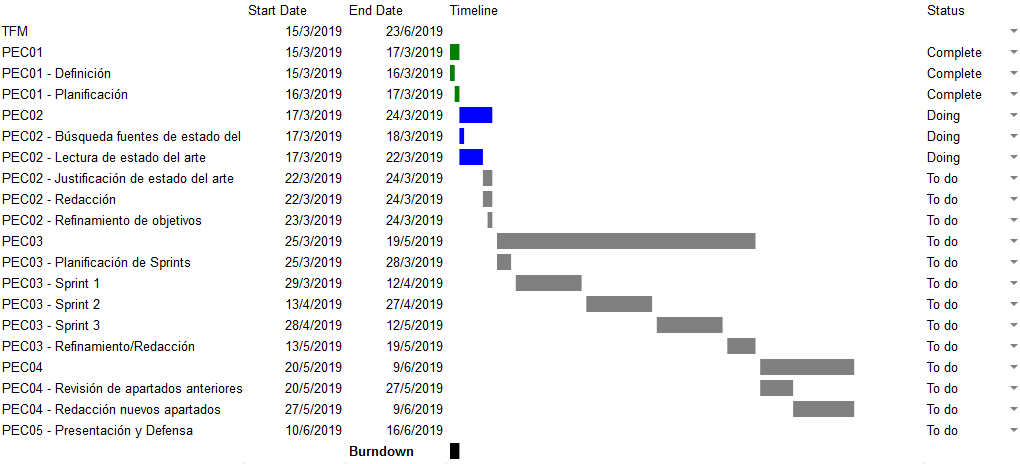
\includegraphics[width=1\textwidth]{figs/gantt_init.PNG}
	\caption{Planificación de tareas}
	\label{fig:gantt}
\end{figure}
